\documentclass[11pt,a4paper]{article}
\usepackage[margin=1in]{geometry}
\usepackage{hyperref}

\usepackage{pgfplots}
% \pgfplotsset{width=4in,compat=1.9}
\pgfplotsset{compat=1.17}

\usepackage{float}
% Figure layout
\usepackage{subcaption}
\captionsetup{font={small}}


\begin{document}


\begin{titlepage}

    % You need to edit the details here

    \begin{center}
        {\LARGE University of Sheffield}\\[1.5cm]
        \linespread{1.2}\huge {\bfseries Assignment: Sentiment Analysis of Movie Reviews}\\[1.5cm]
        \linespread{1}
        
\includegraphics[width=5cm]{images/tuoslogo.png}\\[1cm]
        {\large COM3110 Text Processing (AUTUMN 2020--21)}\\[1cm]
        {\Large Boxuan Shan}\\[6cm]
        \large Department of Computer Science\\[1cm]
        \today
    \end{center}

\end{titlepage}

% -------------------------------------------------------------------
% Declaration
% -------------------------------------------------------------------

\newpage
\subsection*{\Large Implementation}

In this assignment, a sentiment analysis program for movie reviews has been implemented, which is based on Naive Bayesian model. It implements three main functions, training, predicting and evaluating. In addition, it can extract feature tokens from the training set. The program contains 8 classes. Its core classes are explained in the following.

The Preprocessor class models the dataset preprocessor, which preprocesses phrases with capitalisation and stop-word removal, as well as converts the sentiment scale in the dataset.

The FeatureProcessor class models the processing of feature tokens, which can be used to rank the tokens based on their sentiment score and produce a feature token set, as well as filtering the tokens in a phrase according to the feature token set. The sentiment score measures the sentiment strength of a token, with a high score meaning a strong sentiment bias. The feature token set will be obtained by taking tokens with highest sentiment score. The sentiment score \(u\) for feature token \(t\) is
\setlength{\lineskip}{0em}
\begin{equation}
    u = {(\sum_{s}c(t_i,s)w(s))}^2
\end{equation}

where \(s\) indexing the sentiment over the sentiment scale, \(c(t_i,s)\) is the count of feature token \(t\) within sentiment \(s\). \(w(s)\) is the weight of the sentiment \(s\), neutral sentiment weights 0, positive sentiment weights positive value, negative sentiment weights negative value. The weights of the stronger sentiments get greater absolute value.

The CorpusMeta class models the metadata of the corpus and its extraction process for the training of the dataset. The metadata includes various forms of counting information. The reason for not storing prior probabilities and likelihoods directly is for the compatibility of smoothing algorithms in the Bayesian model.

The Predictor class models the Naive Bayes classifier with Laplace smoothing, which can relies on corpus metadata to predicts the sentiment of a phrase.

% The Predictor class models the Naive Bayesian model, which can relies on corpus metadata to predicts the sentiment of a phrase. The prior probability \(p(s_i)\) of sentiment \(s_i\) is

% \begin{equation}
%     p(s_i) = \frac{c(s_i)}{\sum_{s}c(s)}
% \end{equation}

% where \(c(s_i)\) is the count of feature tokens within the sentiment \(s_i\), \(\sum_{s}c(s)\) is the total feature tokens in the corpus.

% Laplace smoothing is used in the likelihood function, thus, the likelihood \(p(t_j|s_i)\) of feature token \(t_j\) within sentiment \(s_i\)

% \begin{equation}
%     p(t_j|s_i) = \frac{c(t_j,s_i)+1}{c(s_i)+|V|}
% \end{equation}

% where \(c(t_j,s_i)\) is the count of feature token \(t_j\) within sentiment \(s_i\), \(c(s_i)\) is the count of all feature tokens within the sentiment, \(|V|\) is the count of distinct feature tokens in the corpus.

% Therefore, the sentiment \(s^*\) of a phrase is

% \begin{eqnarray}
%     s^* = \mathop{\arg\max}_{s_i} p(s_i) \prod^{N}_{j=1} p(t_j|s_i)
% \end{eqnarray}

% where \(j\) index the feature tokens in the target phrase.

The Evaluator class models the evaluation process, it assesses the accuracy of the predictions of the development set and plots a confusion matrix.

In the training phase, the training set will be loaded with the Phase class, followed by preprocessing with Preprocessing, feature extraction with FeatureProcessor and then training with CorpusMeta. In the prediction phase, the data set will be loaded with the Phase class, then the sentiments of phases will be predicted with Predictor. In the evaluation phase, the accuracy of the predictions will be evaluated with Evaluator and a confusion matrix will be plotted. To use the code, run ``sentiment\_analysis.py -h'' to see startup options and examples.

\subsection*{\Large Evaluation}

A set of movie reviews with a 5-value sentiment label was divided into a training set, a development set and a test set. Firstly, set the feature token as all the tokens in the training set. The programme will be used to train two models on the training set, one using a 5-value sentiment scale and the other using a 3-value sentiment scale. Both models are then used for prediction and evaluation on the development set. Afterwards, adjust the number of extracted feature tokens and repeat the training, prediction and evaluation process. The represention of the number of feature tokens as a ratio relative to all the distinct tokens in the training set.

The confusion matrix for models using 1.0, 0.5 and 0.1 as the feature ratio shown as Figure~\ref{fig:cm}, where 1.0 feature ratio is equivalent to using the all the tokens in the training set as feature tokens.

\begin{figure}[ht]
    \centering
    \begin{subfigure}[t]{0.3\textwidth}
        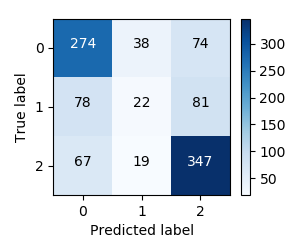
\includegraphics[width=0.8\textwidth]{images/cm3_1.0.png}
        \caption{3-value scale, feature ratio 1.0}
    \end{subfigure}\label{fig:cm310}
    \begin{subfigure}[t]{0.3\textwidth}
        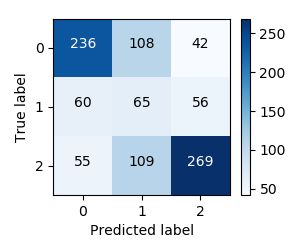
\includegraphics[width=0.8\textwidth]{images/cm3_0.5.png}
        \caption{3-value scale, feature ratio 0.5}
    \end{subfigure}\label{fig:cm305}
    \begin{subfigure}[t]{0.3\textwidth}
        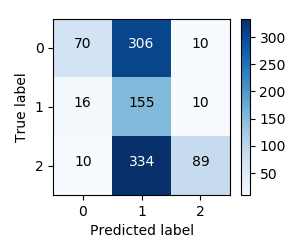
\includegraphics[width=0.8\textwidth]{images/cm3_0.1.png}
        \caption{3-value scale, feature ratio 0.1}
    \end{subfigure}\label{fig:cm301} \\
    \begin{subfigure}[t]{0.3\textwidth}
        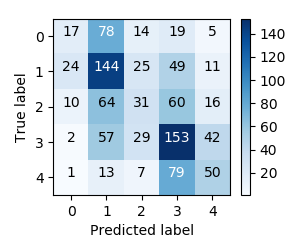
\includegraphics[width=0.8\textwidth]{images/cm5_1.0.png}
        \caption{5-value scale, feature ratio 1.0}
    \end{subfigure}\label{fig:cm510}
    \begin{subfigure}[t]{0.3\textwidth}
        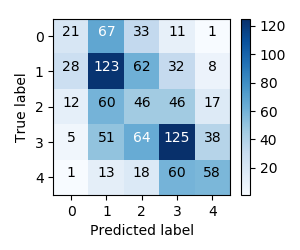
\includegraphics[width=0.8\textwidth]{images/cm5_0.5.png}
        \caption{5-value scale, feature ratio 0.5}
    \end{subfigure}\label{fig:cm505}
    \begin{subfigure}[t]{0.3\textwidth}
        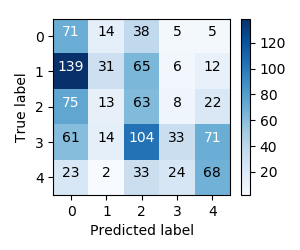
\includegraphics[width=0.8\textwidth]{images/cm5_0.1.png}
        \caption{5-value scale, feature ratio 0.1}
    \end{subfigure}\label{fig:cm501}
    \caption{Confusion matrix under different configurations}\label{fig:cm}
\end{figure}

The feature token ratio was adjusted progressively with a step size of 0.001 to evaluate the model accuracy on the development set. The accuracy profile is shown as Figure~\ref{fig:ratio}. Two sentiment scales produced 200 models in total. The best accuracy was obtained when the feature token ratio was 1.0, where accuracy is 0.643 for the 3-value sentiment scale and 0.395 for the 5-value sentiment scale.

\begin{figure}[ht]
    \centering
    \begin{tikzpicture}[scale=0.55]
        \begin{axis}[
                title={Accuracy dependence of feature set size},
                xlabel={Size ratio of the feature token set},
                ylabel={Prediction accuracy},
                legend pos=north west,
                xtick={0, 0.1, ..., 2.0},
                ytick={0, 0.1, ..., 2.0},
                xmin = 0,
                xmax = 1,
                grid=both,
                height=0.4\textwidth,
                width=0.8\textwidth,
            ]

            \addplot[color=blue, mark=x] table {data/auto_eval_3_12063.txt};
            \addlegendentry{3-value scale}

            \addplot[color=red, mark=x] table {data/auto_eval_5_12063.txt};
            \addlegendentry{5-value scale}

        \end{axis}
    \end{tikzpicture}
    \caption{Model accuracy over different size of feature token set}\label{fig:ratio}
\end{figure}

\subsection*{\Large Analysis}

The accuracy of the classification is not very high, where 0.643 for the 3-value sentiment scale and 0.395 for the 5-value sentiment scale. This probably because Naive Bayesian classifier assumes that all features are independent, however, there are contextual relationships in the text, therefore this assumption is not fully applicable to text classification.

From Figure 1, it is clear that when take 1.0 as the feature ratio, that is, taking all the word tokens from the training set as feature tokens, there are relatively accurate classification results for both sentiment scales. When taking 0.5 as the feature ratio, the model's predictions still reflect an similar sentiment distribution to the ground true. This is benefited by the prior probability in the Naive Bayesian classifier, which allows relatively accurate predictions based on the general sentiment distribution in the training set, when partial likelihood information in a phrase is missing. When taking 0.1 as the feature ratio, the model's predictions reflect an almost opposite distribution due to the effect of Laplace smoothing. In the absence of a large amount of feature token counts, Laplace smoothing will tend to take a lower features' likelihood for sentiments with higher priori probability. This results in sentiments with a high prior probability will have a lower posterior likelihood, which is against the concept of Naive Bayes.

From Figure 2, it is clear that the decline in accuracy is approximately logarithmic with the decline in the count of feature tokens, thus halving the number of feature tokens only slightly reduces the accuracy of the model predictions, whereas the footprint of the model file can be halved. This can be seen as a trade-off between model footprint and classification accuracy in the model optimisation.

\end{document}
